\section{Исследование алгоритмов и адаптивных моделей компенсации нелинейных искажений в передатчике устройств связи} \label{sec:dpd_exp}

% Привязка нумерации формул к секциям/подсекциям/главам
%\numberwithin{equation}{section}
\numberwithin{equation}{subsection}
%\numberwithin{equation}{chapter}

Усилители мощности (УМ) вносят нелинейные искажения, которые существенно влияют на качество радиочастотных сигналов, приводя к ухудшению характеристик передаваемого сигнала. Искажения, вносимые УМ, могут быть классифицированы как внутриполосные и внеполосные.

В случае отсутствия методов линеаризации передающего тракта нелинейные искажения приводят к увеличению вероятности битовой ошибки (BER) на приёмной стороне, возникновению кобминационных помеховых составляющих, а также к ухудшению качества передачи сигналов в соседних частотных каналах. 

Для компенсации нелинейных искажений в современных базовых станциях и пользовательских устройствах широко применяется метод цифровой предыскажения (Digital Pre-Distrotion -- DPD)~\cite{dpd_models, GuoYan_PA_DPD_2015, GuoYan_PA_DPD_Poly}.

Система DPD реализуется в виде блока с обратной нелинейной характеристикой, который реализует предварительное преобразование входного сигнала усилителя мощности с целью минимизации нелинейных искажений на выходе УМ (рис.~\ref{fig:dpd_structure}). Постановка задачи оптимизации метода цифрового предыскажения подробно описана в разделе~\ref{subsec:dpd_describtion} главы~\ref{chapter:intro}.

\subsection{Компенсация нелинейных искажений в передатчике устройств связи в условиях динамического изменения выходной мощности нелинейного усилителя} \label{subsec:dynamic_dpd_2d}

Фундаментальным условием корректного функционирования системы цифрового предыскажения является предположение о стационарности нелинейных искажений, а также исходного сигнала передатчика~\cite{dpd_models}. Сходимость алгоритмов адаптации модели цифрового предыскажения~\eqref{dpd_task_simplif} основана на допущении, согласно которому входной и опорный сигналы формируются одной и той же стационарной статистической моделью, то есть принадлежат одному и тому же распределению. В условиях нестационарности входных данных и/или опорных сигналов нарушаются предпосылки корректного обучения, что, как следствие, приводит к отсутствию сходимости алгоритма адаптации~\cite{widrow1985adaptive}.

Тем не менее, в системах связи для выполнения заданных требований ресурсные блоки (RB) в составе кадра данных могут динамически распределяться в зависимости от текущей нагрузки трафика. Это приводит к кратковременным изменениям уровня мощности, что, в свою очередь, снижает эффективность работы усилителя мощности. Данное обстоятельство противоречит предположению о стационарном режиме функционирования системы цифрового предыскажения. Указанная проблема была рассмотрена в работе~\cite{Dynamic_DPD_RB_Alloc}.

С другой стороны, для повышения энергетической эффективности требуется существенное изменение уровней входной мощности усилителя мощности. В зависимости от класса базовой станции стандартные спецификации 3GPP/ETSI предписывают различные пределы выходной мощности: для Medium Range устройств до $\approx$+38 dBm, для Local Area — около $\approx$+24 dBm, и для домашних станций — до $\approx$+20 dBm на один передатчик. Соответственно, динамический диапазон регулировки выходной мощности может достигать 20–30 дБ относительно максимума, что существенно влияет на нелинейные характеристики усилителей мощности и требует адаптивных методов линейзации~\cite{etsi_ts_136104}. Для компенсации искажений, вызванных изменениями мощности, система цифрового предыскажения должна быть перенастроена в реальном времени, что на практике зачастую оказывается экономически нецелесообразным.

Кроме того, переходные процессы, возникающие при переключении режимов выходной мощности усилителя, приводят к дополнительным искажениям, распространяющимся по каналу связи. Это вызывает кратковременные нарушения протоколов связи и ухудшению спектральной маски. Как следствие, модель цифрового предыскажения, обученная для статического режима выходной мощности УМ, теряет эффективность при обработке сигналов с иным уровнем выходной мощности. Данный эффект наглядно демонстрируется анализом мгновенной спектральной плотности мощности, представленным на рис.~\ref{fig:psd_instat}.

\begin{figure}[ht!]
	\centering
	\begin{subfigure}[b]{0.48\textwidth}
		\centering
		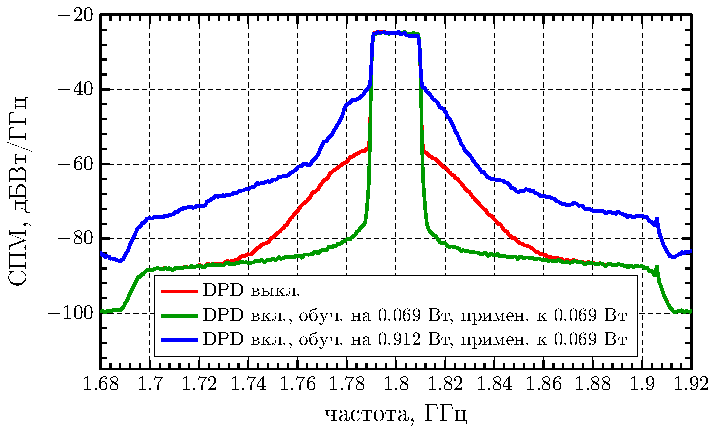
\includegraphics[width=\linewidth]{figures/results/dpd_dynamic_2d/dynamic/PSD_train_test_0p069W.pdf}
		\captionsetup{justification=centering}
		\caption{Применение одномерной модели. Обучение при мощности 0.912~Вт, тестирование при мощности 0.069~Вт}
		\label{fig:psd_high2low_high_range}
	\end{subfigure}
	\hfill % Вместо \hspace{0.3cm} - автоматическое заполнение пространства
	\begin{subfigure}[b]{0.48\textwidth}
		\centering
		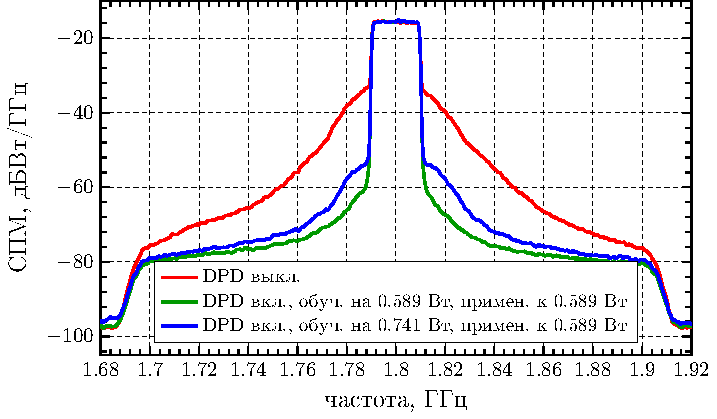
\includegraphics[width=\linewidth]{figures/results/dpd_dynamic_2d/dynamic/PSD_train_test_0p589W.pdf}
		\captionsetup{justification=centering}
		\caption{Применение одномерной модели. Обучение при мощности 0.741~Вт, тестирование при мощности 0.589~Вт}
		\label{fig:psd_high2low_low_range}
	\end{subfigure}
	
	\captionsetup{justification=centering}
	\caption{Спектральная плотность мощности на выходе усилителя. Иллюстрация нестационарности при динамическом изменении режимов мощности}
	\label{fig:psd_instat}
\end{figure}

На рис.~\ref{fig:psd_high2low_high_range} параметры одномерной полиномиальной модели~\eqref{nonlin_pa_out_polinom}, обученные для случаев выходной мощности 0.069~Вт (зелёная кривая) и 0.912~Вт (синяя кривая), применяются к сигналу с выходной мощностью 0.069~Вт. Можно наблюдать ухудшение коэффициента утечки в соседний канал ACLR~\eqref{aclr_criterion} до 32~дБ, обусловленное различиями в поведении нелинейной характеристики усилителя мощности при выбранных режимах.

В то же время, при обучении модели на близких значениях выходной мощности усилителя, а именно 0.598~Вт (зелёная кривая) и 0.714~Вт (синяя кривая) (рис.~\ref{fig:psd_high2low_low_range}), ухудшение компенсации внеполосных искажений составляет 7.5~дБ.

В результате усиленные нелинейные искажения могут распространяться по каналу связи в процессе адаптации параметров модели. В связи с этим более предпочтительным является подход, ориентированный на предсказание нелинейных искажений для всех рабочих режимов усилителя мощности, а не на отслеживание отдельных уровней выходной мощности.

Одним из методов предсказания нелинейных искажений, обусловленных различными режимами мощности усилителя, являются методы пересчёта параметров модели относительно выбранного опорного режима.

Так, в работе~\cite{GuoYan_PA_DPD_2015} предложено разделение обучаемых параметров модели на статическую и динамическую составляющие, при этом динамические параметры переключаются в зависимости от режима мощности усилителя. В работе~\cite{GuoYan_PA_DPD_Poly} данная концепция была расширена путём применения модели адаптивного поворота векторного разложения (power-adaptive decomposed vector rotation, PDVR).

Другой класс методов основан на использовании алгоритмов искусственного интеллекта~\cite{Dynamic_DPD_ANN, Dynamic_DPD_CNN}. В частности, в работе~\cite{Dynamic_DPD_ANN} предлагается использовать нейронную сеть для извлечения признаков, связанной с различными типами нелинейностей, и последующего преобразования параметров обобщённой полиномиальной модели с памятью~\cite{dpd_models} в параметры, соответствующие требуемому уровню мощности, что позволяет прогнозировать нелинейное поведение усилителя мощности для заданного режима.

В данном разделе предлагается альтернативный метод предсказания нелинейных искажений в условиях динамически изменяющейся выходной мощности усилителя, основанный на адаптации двумерного полинома Чебышёва. По сути, данный подход представляет собой классический метод, в котором динамические условия учитываются за счёт использования дополнительных признаков, соответствующих различным режимам работы УМ.

Отметим, что функция потерь для задачи цифрового предыскажения для динамического режима работы УМ состоит из суммы элементарных функций потерь~\eqref{dpd_task_simplif}, соответствующих различным режимам:
\begin{equation}
	\dsp J=\sum_{i=0}^{C-1}\left\lVert f(\bit{x}, \bit{p}, \bit{h}) - \bit{e}_i \right\rVert_2^2 \rightarrow \dsp\min_{\bit{h}},
	\label{dpd_task_simplif_dynamic}
\end{equation}
где $C$ — количество режимов выходной мощности усилителя, $\bit{p}\in\mathbb{C}^{N\times1}$ — вектор признаков входной мощности усилителя. Таким образом, пара $(\bit{x}, \bit{p})$ образует двумерный вход модели, а $\bit{h}\in\mathbb{C}^{K\times1}$ является вектором параметров модели цифрового предыскажения.

Классической моделью нелинейных искажений является полиномиальная модель на основе полиномов Чебышева 1-го рода~(раздел~\ref{subsec:polynom_descript} главы~\ref{chapter:intro}):
\begin{align}
	\displaystyle &y_n=\sum_{d=-D}^{D}\sum_{i=0}^{P_1-1}h_{k, i}x_{n-d}T_{i}(|x_{n-d}|), \nonumber \\
	&T_{i}(|x_{n-d}|)=\cos(i\arccos(|x_{n-d}|))
	\label{1d_cheby_nonlin_multibranch}
\end{align}
где $B=2D+1$-- количество ветвей модели, $T_{i}(\cdot)$, $i=\overrightarrow{0, P_1-1}$ -- функциональный базис. Базис Чебышева 1-го рода позволяет увеличить обусловленность задачи. Отметим, что для учёта инерционных свойств УМ модель~\eqref{1d_cheby_nonlin_multibranch} включает в себя сумму нелинейных функций -- ветвей, каждая из которых обрабатывает задержанный сигнал $|x_{n-d}|$, где $d$ — задержка сигнала, соответствующая $d$-й ветви модели. 

Заметим, однако, что классическая одномерная (1D) модель~\eqref{1d_cheby_nonlin_multibranch} не обладает достаточной обобщающей способностью для описания дианмического режима работы УМ (рис.~\ref{fig:psd_instat}). В связи с этим предлагается двумерная (2D) нелинейная модель, входными признаками которой являются амплитуда сигнала $|x_n|$, а также признак, отражающий текущий режим мощности УМ $p_n$. Признак $p_n$ соответствует входной мощности УМ, равномерно возрастающей в линейном масштабе. Всего рассматривается $61$ уровень мощности~\eqref{input_powers_dbm}, описанных в разделе~\ref{subsec:data_dpd_dynamic} главы~\ref{chapter:methods}.

\begin{figure}[!ht]
	\centering
	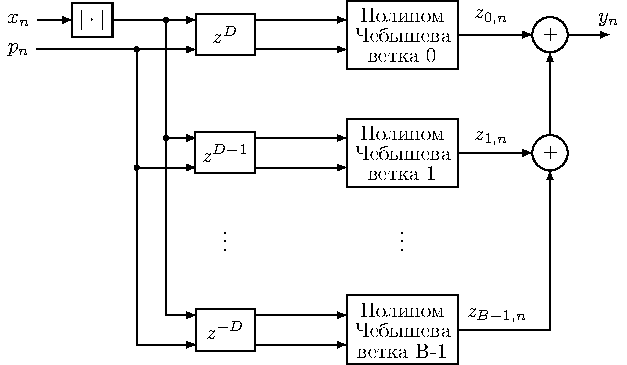
\includegraphics[width=0.75\linewidth]{figures/results/dpd_dynamic_2d/cheby_scheme/Cheby_poly_model.pdf}
	\captionsetup{justification=centering}
	\caption{Двумерная модель компенсации нелинейных искажений в условиях динамического режима работы УМ на основе полиномов Чебышева 1-го рода}
	\label{fig:cheby_scheme}
\end{figure}

Предлагаемая двумерная полиномиальная модель изображена на рис.~\ref{fig:cheby_scheme} и представляет собой следующее выражение:
\begin{align}
	\displaystyle y_n&=\sum_{d=-D}^{D}\sum_{i=0}^{P_1-1}\sum_{j=0}^{P_2-1}h_{i, j, d}x_{n-d}T_{i, j}(|x_{n-d}|, p_{n-d}), \nonumber \\
	\displaystyle T_{i, j}(|x_n|, p_n)&=T_{i}(|x_n|)T_{j}(p_n)=\cos(i\arccos(|x_n|))\cos(j\arccos(p_n)),
	\label{dpd_model_2d}
\end{align}
где $B=2D+1$ -- число веток модели, $P_1$, $P_2$ — порядки двумерного полинома Чебышёва по измерениям амплитуды сигнала и режима мощности соответственно, $\displaystyle\{h_{i,j}\}_{i=0,j=0}^{P_1-1,P_2-1}$ — настраиваемые параметры двумерного полинома. Базисные функции двумерной нелинейности $T_{i, j}(\cdot)$ выражаются через произведение одномерных базисных функций $T_{i}(\cdot)$ и $T_{j}(\cdot)$, соответствующих амплитуде сигнала и мощности УМ. Отметим, что амплитуда входного сигнала $|x_n|$ и признак режима УМ $p_n$ нормируются в единый диапазон $[-1, 1]$ как для стандартизации данных, так и для выполнения условий ортогональности полиномов Чебышёва.

Модель~\eqref{dpd_model_2d} обучается на $C=31$~\eqref{dpd_task_simplif_dynamic} сигнале, которые соответствуют четным элементами последовательности~\eqref{input_powers_dbm}. Таким образом обучение модели производится на данных, соответствующие входной мощности $p_n$:
\begin{subequations}\label{input_powers_even}
	\begin{align}
		&25.1 \text{ мкВт}, \text{ }50.8\text{ мкВт}, \cdots, 794.3 \text{ мкВт} \nonumber \\
		&14.0 \text{ дБмк}, \text{ }17.1\text{ дБмк}, \cdots, 29.0 \text{ дБмк},
	\end{align}
\end{subequations}
а также выходной мощности УМ:
\begin{align}
	&0.069 \text{ }\text{Вт}, \text{ }0.143\text{ }\text{Вт}, \cdots, 0.912 \text{ }\text{Вт} \nonumber \\
	-&11.6\text{ дБВт},-8.4\text{ дБВт}, \cdots,-0.4\text{ дБВт} 
	\label{powers_all_even}
\end{align}

В данном разделе производится сравнение обощающей способности 2-х моделей~\eqref{1d_cheby_nonlin_multibranch},~\eqref{dpd_model_2d}. Параметры обеих моделей представлены в таблице~\ref{table:dpd_dynamic_param_table}.
\begin{table}[htbp]
	\centering
	\begin{tabular}{|c|c|c|c|c|}
		\hline
		Модель & Число веток $B$ & Порядок $P_1$ & Порядок $P_2$ & Число параметров \\
		\hline
		1D-полином~\eqref{1d_cheby_nonlin_multibranch}  & 37  & 24  & --- & 888 \\
		\hline
		2D-полином~\eqref{dpd_model_2d}  & 9  & 8  & 12  & 864 \\
		\hline
	\end{tabular}
	\caption{Параметры моделей компенсации нелинейных искажений в условиях динамического изменения режима УМ}
	\label{table:dpd_dynamic_param_table}
\end{table}

Поскольку моделий~\eqref{1d_cheby_nonlin_multibranch},~\eqref{dpd_model_2d} линейные по параметрам и, как следствие, функция потерь~\eqref{mse_block} является квадратичной, то глобальный оптимум в обоих случаях может быть найден методом LS~\eqref{ls_eq_jac} за один шаг (раздел~\ref{subsec:ls} главы~\ref{chapter:intro}). Будем адаптировать модели при помощи метода LS, а также ускоренного при помощи оптимизатора Adam блочного градиентного спуска (раздел~\ref{subsec:grad_modified} главы~\ref{chapter:intro}). 

Метод LS адаптирует модель на полном массиве тренировочных данных длиной $31\cdot147384=4568904$ отсчетов. При этом стохастическая версия градиентного спуска обучается модели на матрице данных размерности $31\times 267$, где блоки длиной 267 выбираются из массивов соответствующих различным режимам УМ~\eqref{input_powers_even}. Всего $147384 / 267=552$ блоков на всю тренировочную выборку. Градиенты~\eqref{grad_descent_сomplex_mse_holomorphic}, посчитанные на блоках для разных режимов УМ агрегируются для пересчета параметров модели:
\begin{equation}
	\bit{z}_{k+1}=\bit{z}_{k}+\frac{\mu}{C}\sum_{i=0}^{C-1}(D_{\bit{z}}\bit{y}_i)^H\bit{e}_i.
	\label{grad_descent_agregate_dynamic}
\end{equation}
Такой способ формирования обучающих блоков данных обеспечивает равномерное усвоение параметрами модели информации, соответствующей данным с различными статистическими характеристиками.

Якобианы $D_{\bit{z}}\bit{y}_i$, $i=\overrightarrow{0, C-1}$~\eqref{grad_descent_agregate_dynamic} для метода градиентного спуска и метода LS для адаптации двумерной модели~\eqref{dpd_model_2d} вычисляются в соответствии с формулами~\eqref{jac_2d_model_full}.

Порядок полинома Чебышёва~$P_2$ (таблица~\ref{table:dpd_dynamic_param_table}) выбран таким образом, чтобы обеспечить приемлемые значения коэффициента утечки в соседний канал (ACLR) было на уровне не хуже $-50\text{ дБ}$ во всём диапазоне режимов работы УМ.

Общее число параметров одномерной модели выбрано примерно равным числу параметров двухмерной модели (таблица~\ref{table:dpd_dynamic_param_table}) с целью обеспечения корректного сравнения.

\begin{figure}[!b]
	\centering
	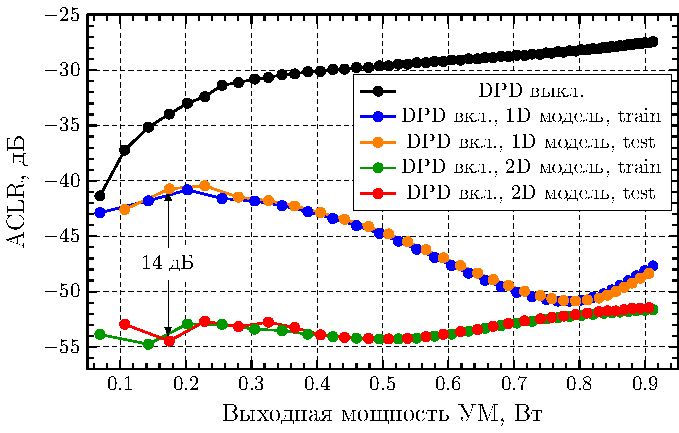
\includegraphics[width=0.7\linewidth]{figures/results/dpd_dynamic_2d/perform/performance.pdf}
	\captionsetup{justification=centering}
	\caption{Уровень компенсации внеполосных искажений в передатчике устройства связи засчет адаптации 1D- и 2D-моделей на основе полиномов Чебышёва 1-го рода}
	\label{fig:perform_all_data_dynamic}
\end{figure}

\begin{figure*}[ht]
	\centering
	\begin{subfigure}[b]{0.48\textwidth}
		\centering
		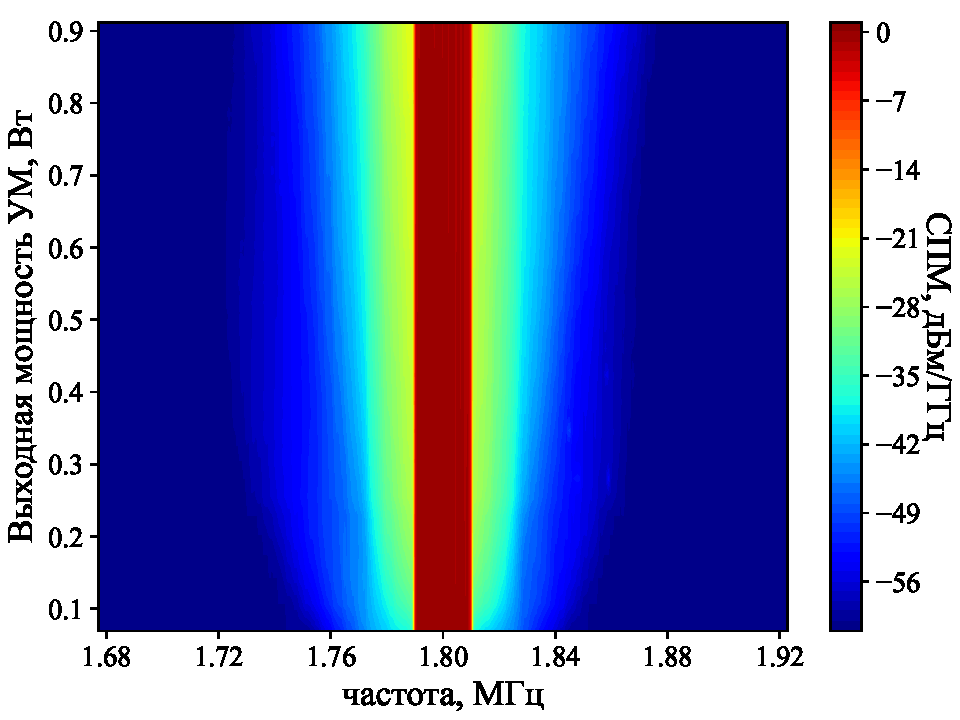
\includegraphics[width=\linewidth]{figures/results/dpd_dynamic_2d/analyze/plot_graphs/psd/PSD_not_corrected_all_powers_cmap.pdf}
		\captionsetup{justification=centering}
		\caption{DPD выкл.}
		\label{fig:psd_not_corrected_cmap}
	\end{subfigure}
	\hfill
	\begin{subfigure}[b]{0.48\textwidth}
		\centering
		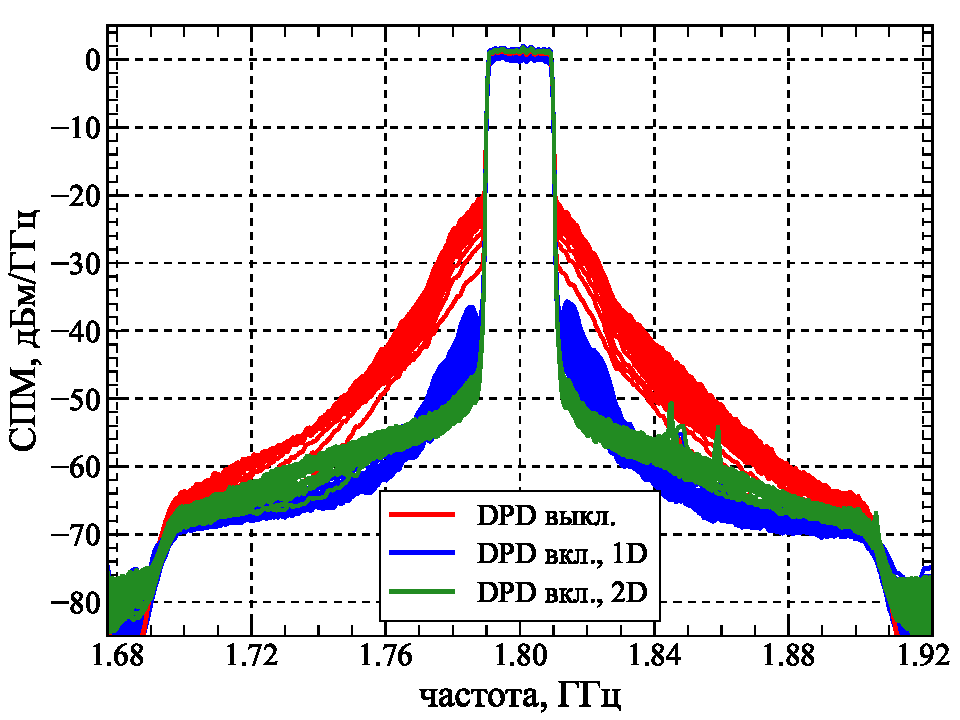
\includegraphics[width=0.95\linewidth]{figures/results/dpd_dynamic_2d/analyze/plot_graphs/psd/PSD_corrected_NC_1d_2d_all_powers.pdf}
		\captionsetup{justification=centering}
		\caption{DPD выкл./вкл., 1D- и 2D-модели на основе полиномов Чебышёва 1-го рода}
		\label{fig:psd_1d_and_2d_corrected}
	\end{subfigure}
	
	\vskip\baselineskip
	
	\begin{subfigure}[b]{0.48\textwidth}
		\centering
		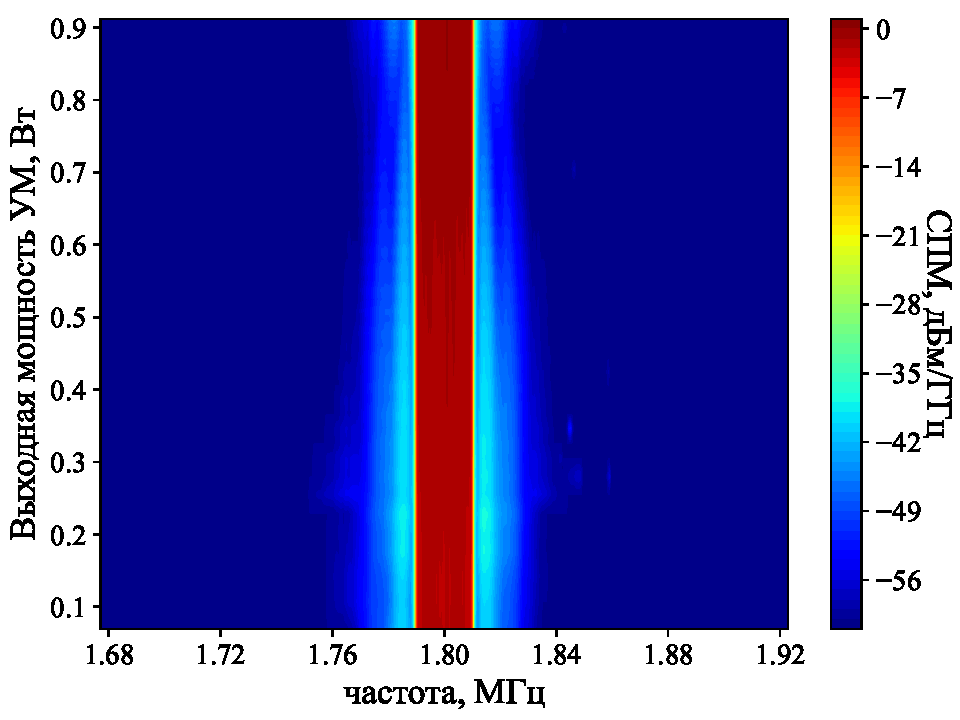
\includegraphics[width=\linewidth]{figures/results/dpd_dynamic_2d/analyze/plot_graphs/psd/PSD_corrected_1d_all_powers_cmap.pdf}
		\captionsetup{justification=centering}
		\caption{DPD вкл., 1D-модель}
		\label{fig:psd_1d_corrected_cmap}
	\end{subfigure}
	\hfill
	\begin{subfigure}[b]{0.48\textwidth}
		\centering
		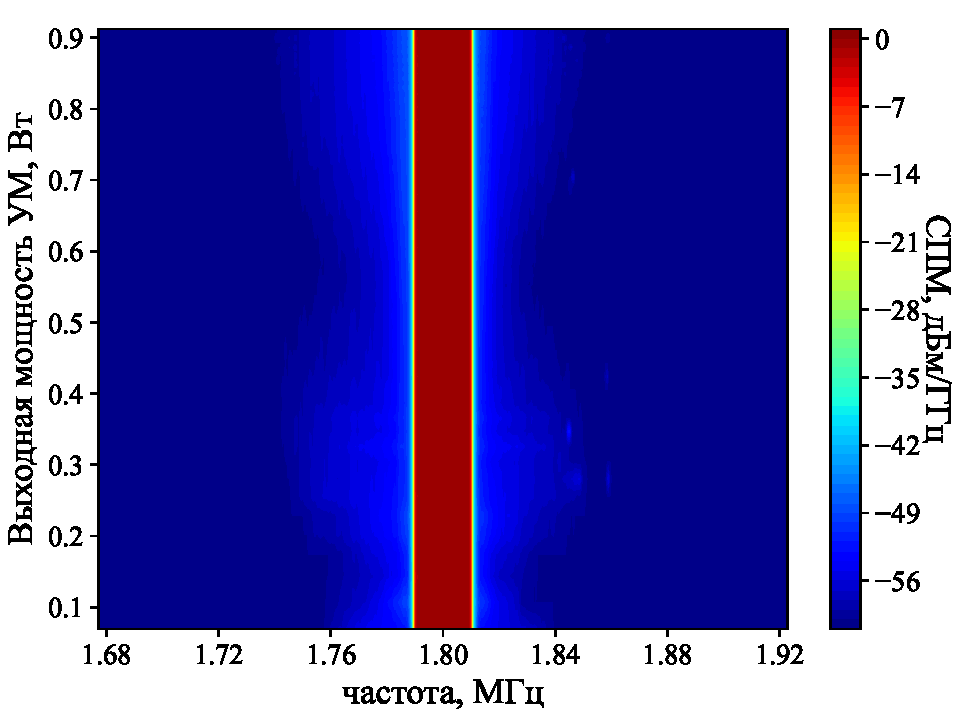
\includegraphics[width=\linewidth]{figures/results/dpd_dynamic_2d/analyze/plot_graphs/psd/PSD_corrected_2d_all_powers_cmap.pdf}
		\captionsetup{justification=centering}
		\caption{DPD вкл., 2D-модель}
		\label{fig:psd_2d_corrected_cmap}
	\end{subfigure}
	
	\caption{СПМ сигнала на выходе УМ. Результат применения 1D- и 2D-моделей на основе полиномов Чебышева 1-го рода}
	\label{fig:psd_dynamic}
\end{figure*}

Уровень компенсации обеих моделей представлен на рис.~\ref{fig:perform_all_data_dynamic}. Согласно результатам численных экспериментов, двухмерная модель обеспечивает уровень $\text{ACLR}<-50\text{ дБ}$ во всём диапазоне выходных мощностей усилителя мощности. Более того, по сравнению с одномерной полиномиальной моделью достигается улучшение ACLR до 14 дБ для всех рассмотренных режимов выходной мощности усилителя.

На рис.~\ref{fig:psd_dynamic} представлены спектральные плотности мощности сигнала передатчика до применения нелинейного корректора и после коррекции с использованием предварительно обученных одномерной и двухмерной моделей на основе полиномов Чебышёва. Оценка качества компенсации внеполосных искажений выполнена как на обучающей, так и на тестовой выборках, при этом соответствующие спектральные плотности мощности выходного сигнала усилителя мощности приведены на рис.~\ref{fig:psd_dynamic}.

На рис.~\ref{fig:psd_not_corrected_cmap} показана цветовая шкала спектральной плотности мощности сигнала передатчика до применения нелинейного корректора для всех рассматриваемых значений выходной мощности усилителя. В свою очередь, на рис.~\ref{fig:psd_1d_corrected_cmap} и \ref{fig:psd_2d_corrected_cmap} приведены цветовые шкалы спектров сигнала на выходе УМ при включенном блоке DPD на основе одномерной и двухмерной моделей Чебышёва соответственно. Дополнительно, на рис.~\ref{fig:psd_1d_and_2d_corrected} представлены СПМ сигнала передатчика до и после применения нелинейной коррекции на одном графике с нормированными уровнями выходной мощности для различных режимов работы УМ.

Таким образом, согласно рис.~\ref{fig:perform_all_data_dynamic}, \ref{fig:psd_1d_corrected_cmap} и \ref{fig:psd_2d_corrected_cmap}, двумерная модель цифровых предыскажений~\eqref{dpd_model_2d} обеспечивает существенное увеличение уровня компенсации внеполосных искажений по сравнению с одномерной моделью~\eqref{1d_cheby_nonlin_multibranch}, достигающее 14 дБ, во всём динамическом диапазоне выходной мощности усилителя: $0.069 \text{ Вт}, \cdots, 0.912 \text{ Вт}$.

Результаты демонстрируют существенное повышение обобщающей способности двумерной модели~\eqref{dpd_model_2d} относительно классического одномерного подхода~\eqref{1d_cheby_nonlin_multibranch}. Данное улучшение обусловлено введением дополнительного измерения, параметризующего текущий мощностный режим работы усилителя мощности.

Такая параметризация позволяет модели предсказывать нелинейные искажения в условиях динамического изменения мощности входного сигнала. Следовательно, устраняется необходимость калибровки и пересчёта параметров модели для различных режимов работ УМ, что в свою очередь минимизирует вероятность кратковременных нарушений протокола связи, вызванных процедурами перенастройки цифрового предыскажения.

Рассмотрим скорость сходимости ускоренного градиентного спуска с оптимизатором Adam~(раздел~\ref{subsec:grad_modified} главы~\ref{chapter:intro}). В данном вычислительной эксперименте использовалолсь линейное изменение скорости шага для ускорения обучения модели~\cite{he2016deep}:
\begin{equation}
	\mu_k=\mu_{\text{start}}+\frac{k}{N-1}(\mu_{\text{end}}-\mu_{\text{start}}).
	\label{linear_scheduler_dpd_dynamic}
\end{equation}
где $\mu_{\text{start}}$, $\mu_{\text{end}}$ -- начальное и конечное значение шага обучения. Таким образом, в~\eqref{linear_scheduler_dpd_dynamic} шаг линейно обуывает от $\mu_{\text{start}}=10^{-4}$ до $\mu_{\text{end}}=10^{-7}$. Индекс шага обучения $k=\overrightarrow{0, N-1}$, $N$ -- число шагов обучения $N=552\cdot E=552\cdot 50=27600$, где $E=50$ -- число эпох, т.е. количество прохождений алгоритма обучения по всей длине тренировочной выборки.

На рис.~\ref{fig:adam_dpd_dynamic} изображено сравнение кривой сходимости ускоренного блочного градиентного спуска с уровнем компенсации нелинейных искажений, полученным при помощи адаптации двумерной модели алгоритмом LS.
\begin{figure}[ht!]
	\centering
	\begin{subfigure}[b]{0.48\textwidth}
		\centering
		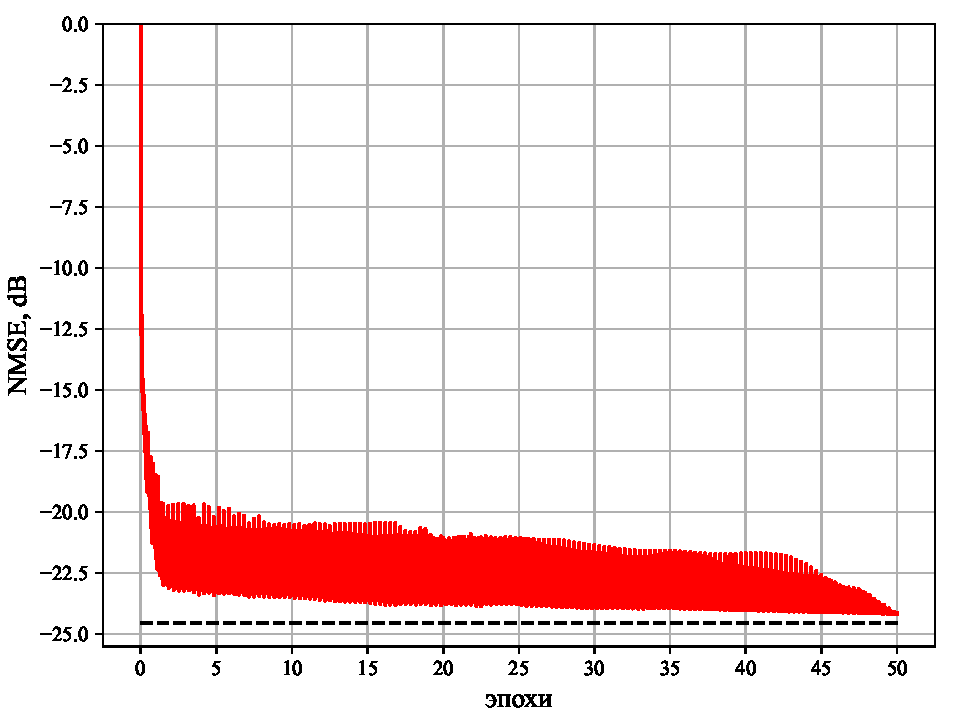
\includegraphics[width=\linewidth]{figures/results/dpd_dynamic_2d/bgd/lc_bgd_full.pdf}
		\captionsetup{justification=centering}
		\caption{}
		\label{fig:adam_dpd_dynamic_normal}
	\end{subfigure}
	\hfill % Вместо \hspace{0.3cm} - автоматическое заполнение пространства
	\begin{subfigure}[b]{0.48\textwidth}
		\centering
		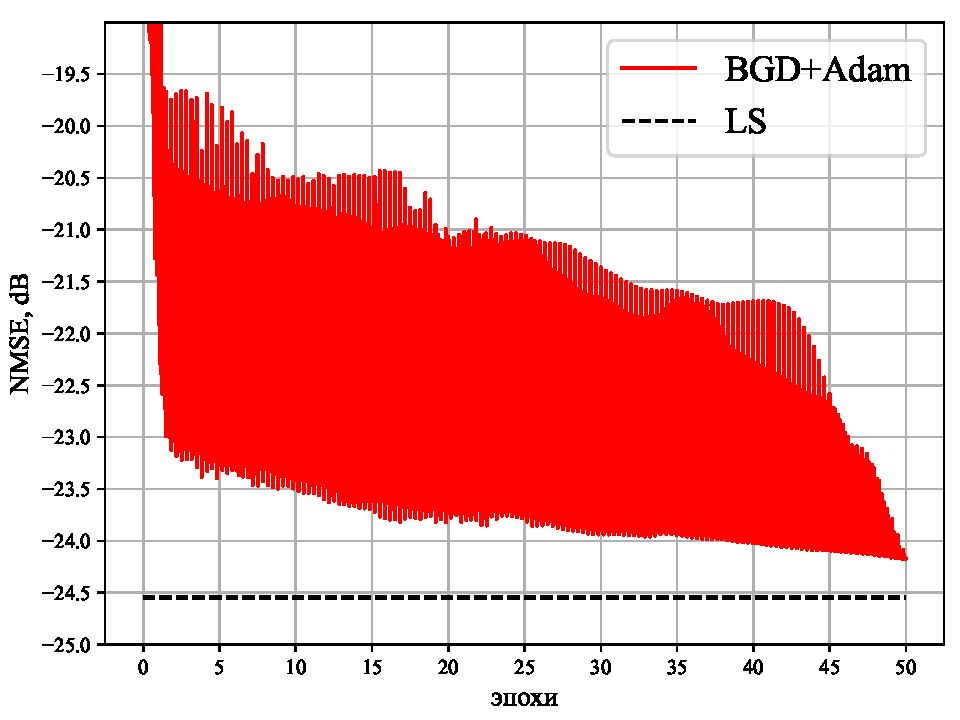
\includegraphics[width=\linewidth]{figures/results/dpd_dynamic_2d/bgd/lc_bgd_expanded.pdf}
		\captionsetup{justification=centering}
		\caption{}
		\label{fig:adam_dpd_dynamic_expanded}
	\end{subfigure}
	
	\captionsetup{justification=centering}
	\caption{Сранение кривой сходимости ускоренного блочного градиентного спуска с уровнем компенсации, полученным при помощи алгоритма LS}
	\label{fig:adam_dpd_dynamic}
\end{figure}

Кривая сходимости, а также уровень компенсации метода LS получен путём подсчета нормированной среднеквадратичной ошибки~\eqref{nmse_block} на всей длине тренировочный данных. При этом в качестве опорного сигнала $\bit{d}$~\eqref{nmse_block} взят исходный сигнал нелинейных искажений на выходе УМ до включения алгоритма адаптации, т.е. разность выхода и входа УМ: $\text{PA}(\bit{x})-\bit{x}$. Таким образом, значения NMSE считаются по формуле:
\begin{equation}
	\text{NMSE}=10\cdot\text{lg}\begin{pmatrix}
		\dsp\frac{\dsp\sum_{i=0}^{C-1}(\text{PA}(\bit{x}_i)-\bit{x}_i-\bit{y}_i)^H(\text{PA}(\bit{x}_i)-\bit{x}_i-\bit{y}_i)}{\dsp\sum_{i=0}^{C-1}(\text{PA}(\bit{x}_i)-\bit{x}_i)^H(\text{PA}(\bit{x}_i)-\bit{x}_i)}
	\end{pmatrix}\text{		}дБ,
	\label{nmse_block_dpd_dynamic}
\end{equation}
где $\bit{x}_i$, $\text{PA}(\bit{x}_i)$, $\bit{y}$ -- вход УМ, выход УМ, выход нелинейной модели соответственно для $i$-ого мощностного режима УМ, $i=\overrightarrow{0, C-1}$, $C=31$ -- число мощностных режимов обучающей выборки~\eqref{powers_all_even}.

На основе рис.~\ref{fig:adam_dpd_dynamic} собрана сравнительная таблица~\ref{table:adam_nmse_epoch_compare_dpd_dynamic} уровня компенсации, полученного в зависимости от числа эпох.
\begin{table}[htbp]
	\centering
	\begin{tabular}{|c|c|c|c|c|}
		\hline
		Метод & 3 эпох & 5 эпох & 27 эпох & 150 эпох \\
		\hline
		BGD+Adam, NMSE дБ  & -21.55  & -22.71  & -23.32 & -24.17 \\
		\hline
		LS, NMSE дБ  & -24.55  & -24.55 & -24.55 & -24.55 \\
		\hline
	\end{tabular}
	\caption{Сравнение уровня компенсации нелинейных искажений методами BGD, LS в зависимости от числа эпох обучения}
	\label{table:adam_nmse_epoch_compare_dpd_dynamic}
\end{table}

Как видно из таблицы~\ref{table:adam_nmse_epoch_compare_dpd_dynamic} ускоренный метод градиентного спуска за 3 эпохи достигает уровня компенсации на 3 дБ меньше оптимального значения, за 5 эпох уровня компенсации $\approx2$ дБ меньше оптимального значения, за 27 эпох на 1.2 дБ меньше оптимального значения. По окончании обучения на 150 эпохах уровень компенсации на $\approx0.4$ дБ меньше уровня компенсации, достигаемого при помощи LS метода. Отличие в 0.4 дБ составляет всего 9.6\% отличия по энергии ошибки. 

\begin{figure}[!h]
	\centering
	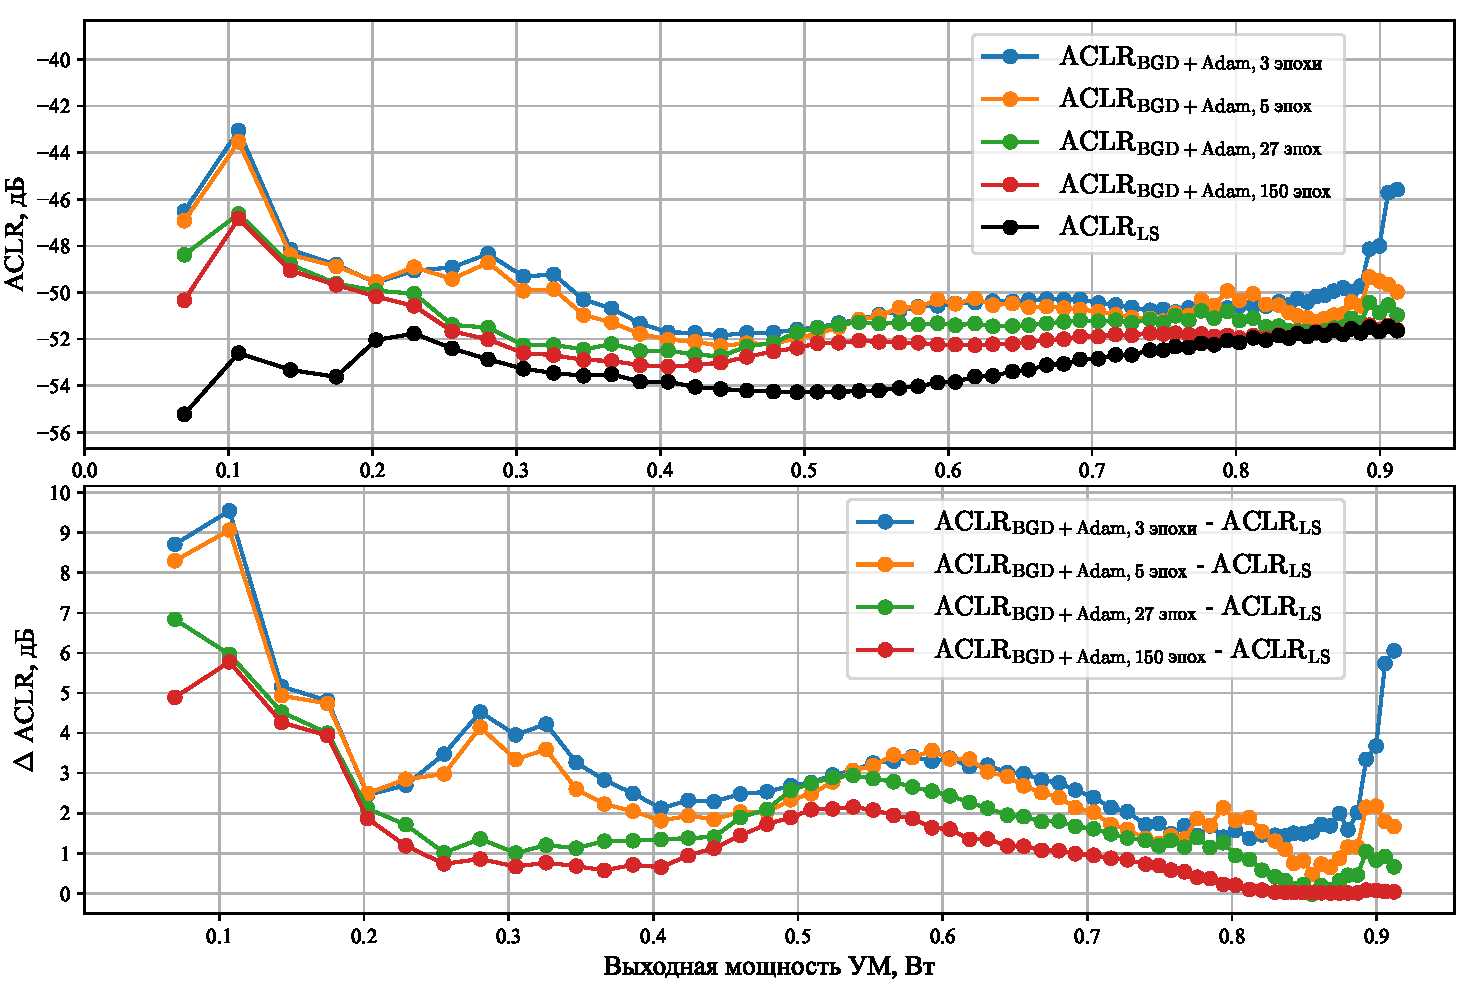
\includegraphics[width=1.0\linewidth]{figures/results/dpd_dynamic_2d/bgd/bgd_vs_ls_2_fig.pdf}
	\captionsetup{justification=centering}
	\caption{Уровень компенсации внеполосных искажений в передатчике устройства связи засчет адаптации двумерной модели методами LS, а также ускоренным методом блочного градиентного спуска при различном числе эпох обучения}
	\label{fig:perform_all_data_dynamic_bgd}
\end{figure}

Тем не менее, уровень компенсации соответствующий отдельным мощностным режимам может существенно отличаться от полученного при помощи метода LS. Это связано с тем, что значения компенсации, отраженные на рис.~\ref{fig:adam_dpd_dynamic} вычисляются по составному критерию~\eqref{nmse_block_dpd_dynamic}, в котором аккумулируется энергия ошибки обучения для всех мощностных режимов тренировочной выборки. При это наибольших вклад в энергию ошибки вносят сигналы сигналы на выходе УМ соответствующие большим значениям выходной мощности. С точки зрения алгоритма адаптации эти сигналы являются наиболее приоритетными. При этом ошибка адаптации, соответствующая меньшим значениям выходной мощности может быть высокой и корректироваться в последнюю очередь.

Этот процесс представлен на рис.~\ref{fig:perform_all_data_dynamic_bgd}. Значения ACLR соответствующие уровню компенсации засчет обучения ускоренным методом градиентного спуска на 5 эпохе для выходной мощности 100 мВт -- на $\approx9.5$ дБ меньше значения, полученного LS-методом, на 10 эпохе для выходной мощности 100 мВт -- на $\approx9$ дБ, на 27 эпохе для выходной мощности 70 мВт -- на $\approx7$ дБ, на 150 эпохе для выходной мощности 100 мВт -- на $\approx6$ дБ.

Представленные результаты демонстрируют необходимость поиска компромиссного метода, который обладает высокой скоростью сходимости, как методы второго порядка и невысокой вычислительной сложностью, как градиентные методы. 

Такой метод предложен в разделе~\ref{subsec:conj_grad} главы~\ref{chapter:implement} и представляет собой адаптацию метода сопряженных градиентов на основе смешанного метода Ньютона (раздел~\ref{subsec:mnm} главы~\ref{chapter:intro}). Предложенный метод обладает сверхлинейной скоросью сходимости и при этом не требует явного обращения матрицы вторых производных.

%Из рис.~\ref{fig:adam_dpd_dynamic} видно, что алгоритм достигает значения $NMSE=-23$ дБ, т.е. на 3 дБ меньше значения, полученного засчет LS, за число эпох равное 10

% Градиентный спуск затронуть. Он уже посчитался
% Возможно нарисовать ACLR(power) для градиентного спуска и сказать что терем перфоманс даже при долгой адаптации. Это поднимает проблему того что хорошо бы использовать методы второго порядка. Они являются дорогими для аппаратной реализации, но в будущем мы предложим метод споряженных градиентов, который является компромиссов между перфомансом и сложностью.

%\subsection{Компенсация нелинейных искажений в передатчике двухканальной системы связи}
%\label{subsec:dpd_2ch_jota}
%
%В данном разделе рассматривается задача компенсации нелинейных искажений, возникающий в передатчике двухканальной системы связи. Проблема формирования комбинационных составляющих в передатчике двухканальной системы, которая описана в разделе~\ref{subsec:data_dpd_2channel} текущей главы. 
%
%Текущий раздел посвящен исследованию различных вариаций метода Ньютона в применении к обучению многослойной нейросетевой комплекснозначной модели. Рассмотрены 4 алгоритма:
%\begin{itemize}
%	\item Метод Ньютона (раздел~\ref{subsec:newton} главы~\ref{chapter:intro}) с адаптивной в регуляризацией на основе алгоритма Левенберга-Марквардта (алгоритм~\ref{alg:lm_adaptive}). Сокращенно NM-LM (Newton Method with Levenberg-Marquardt adaptive regularization control)
%	\label{dpd_2ch_algorithms}
%	\item Кубический метод Ньютона (раздел~\ref{subsec:cubic_nm} главы~\ref{chapter:intro}). Сокращенно CNM (Cubic Newton Method).
%	\item Смешанный метод Ньютона (раздел~\ref{subsec:mnm} главы~\ref{chapter:intro}) с адаптивной в регуляризацией на основе алгоритма Левенберга-Марквардта (алгоритм~\ref{alg:lm_adaptive}). Сокращенно MNM-LM (Mixed Newton Method with Levenberg-Marquardt adaptive regularization control)
%	\item Кубический смешанный метод Ньютона (раздел~\ref{subsec:cubic_mnm} главы~\ref{chapter:intro}). Сокращенно CMNM (Cubic Mixed Newton Method).
%\end{itemize}
%
%Кроме того, производится сравнение эффективности коррекции нелинейных искажений, с также скорости сходимости комплекснозначной и вещественнойзначной моделей.
%
%Сравнение эффективности работы алгоритмов, а также применимости различных моделей к текущей задаче производится на примере компенсации искажений в канале A, изображенном на рис.~\ref{fig:rx_dpd_x_2ch}, \ref{fig:error_dpd_2ch}.
%
%Как было отмечено в разделе~\ref{subsec:2nd_harmonic} текущей главы, нейросетевые модели на основе полносвязного перцептрона (рис.~\ref{fig:mlp}) могут быть интерпретированы как классические нелинейные модели с адаптивными базисными функциями, что позволяет повысить уровень коменсации искажений при том же или меньшем числе адаптивных параметров. В данном разделе предлагается использовать иной вид моделей, представляющих собой сверточную нейронную сеть.
%
%Принципиальным преимуществом сверточных нейронных сетей в контексте нелинейной обработки сигналов является их способность к явному учету инерционности нелинейных преобразований. Архитектура сверточных сетей, основанная на применении временных фильтров, обеспечивает индуктивное смещение в пользу локальных временных зависимостей, что соответствует физической природе сигнальных искажений.
%
%Однако существует несколько популярных подходов к реализации сверточных сетей в задачах нелинейной обработки. Первый подход основан на сведении задачи комплексной обработки к задаче вещественной оптимизации, т.е. обучении модели с вещественными параметрами на вещественных данных. В дальнейшем будем обозначать такую модель как RV-CNN (Real-Valued Convolutional Neural Network).
%
%Второй принципиальный подход заключается в решении задачи оптимиации в комплексной плоскости, т.е. адаптации модели с комплексными параметрами на комплексных данных. Этот подход является более интерпретируемым с физической точки зрения, поэтому, как станет ясно далее, позволяет использовать модель с меньшим числом обучаемых параметров для достижения того же уровня компенсации в сранении с RV-CNN. В дальнейшем будем обозначать такую модель как CV-CNN (Complex-Valued Convolutional Neural Network).
%
%Схемы комплекснозначной и вещественнозначной моделей изображены на рис.~\ref{fig:cv_cnn_dpd_2ch},~\ref{fig:rv_cnn_dpd_2ch} соответственно. 
%\begin{figure}[h!]
%	\centering
%	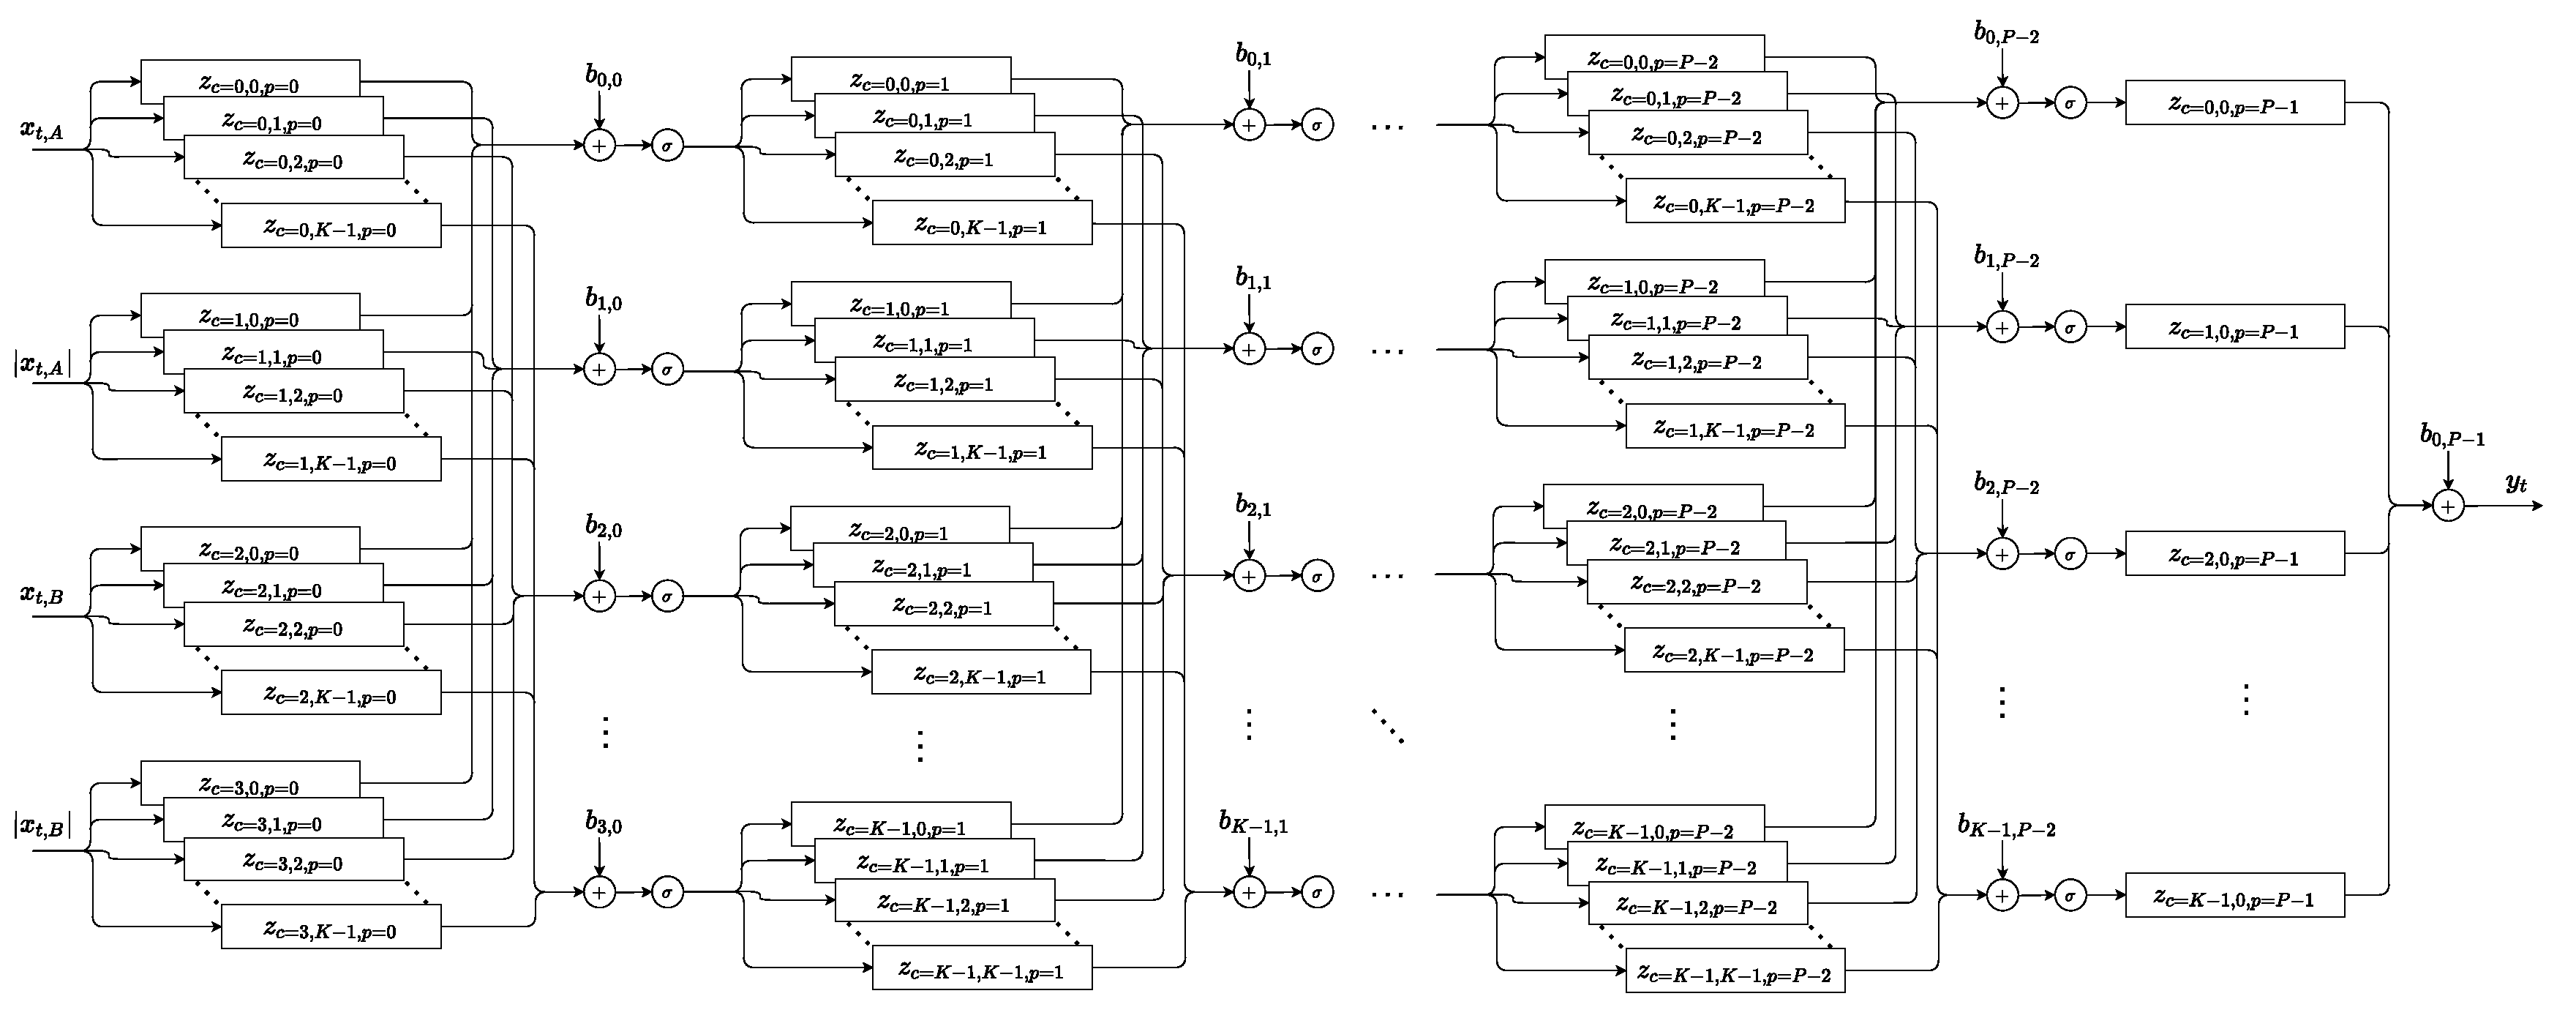
\includegraphics[scale=0.28]{figures/models/cnn/cv_cnn.pdf}
%	\caption{Схема свёрточной нейронной сети с комплексными параметрами CV-CNN на основе одномерных сверточных ядер}
%	\label{fig:cv_cnn_dpd_2ch}
%\end{figure}
%\begin{figure}[h!]
%	\centering
%	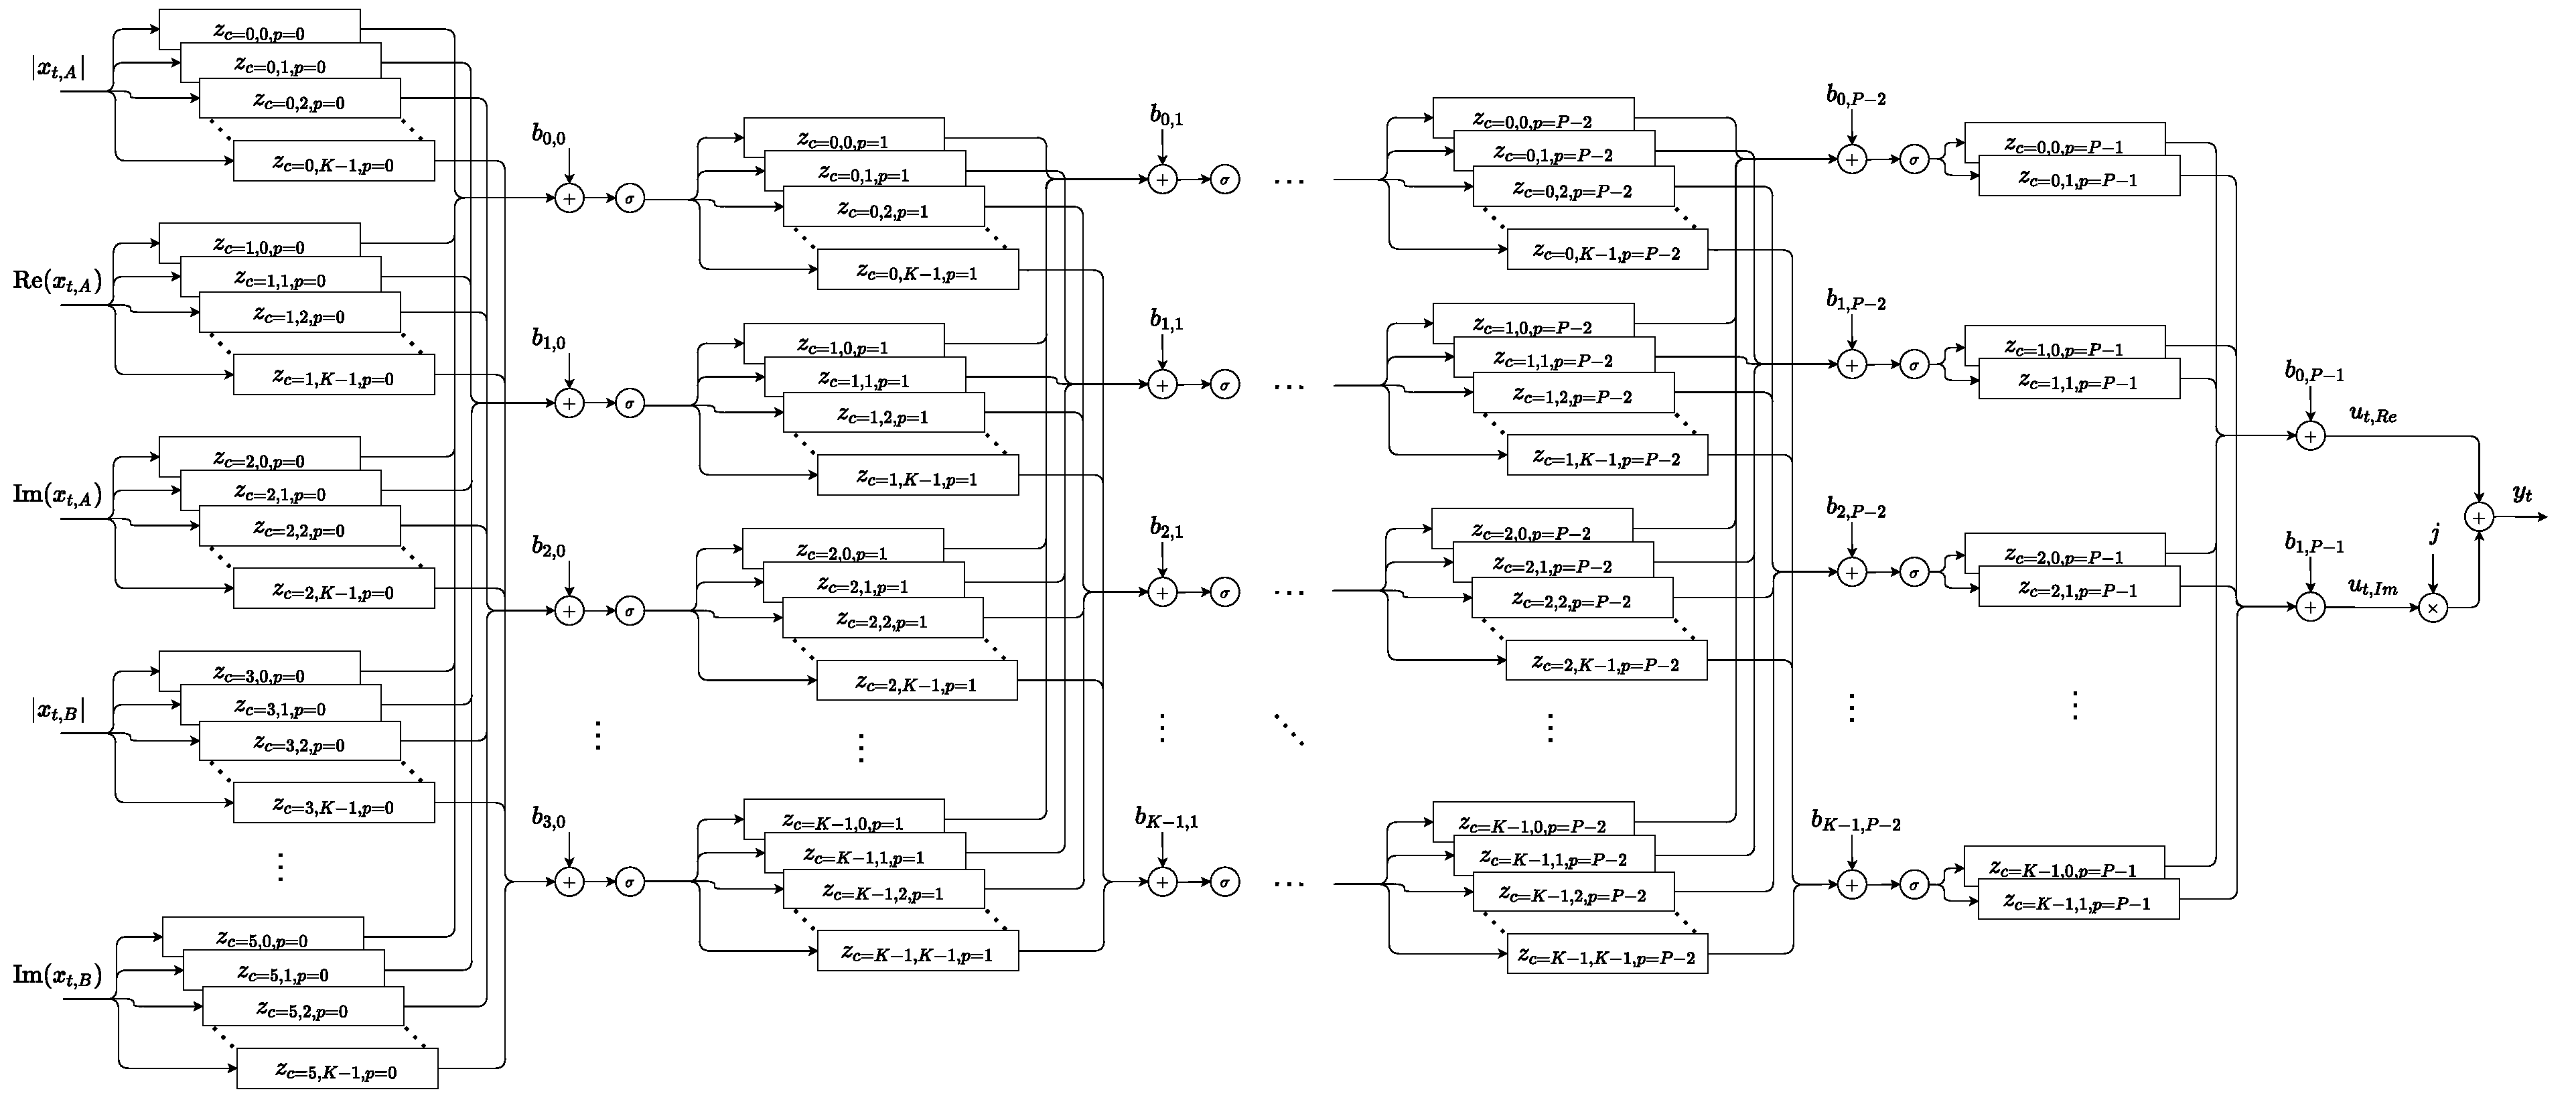
\includegraphics[scale=0.26]{figures/models/cnn/rv_cnn.pdf}
%	\caption{Схема свёрточной нейронной сети с вещественными параметрами RV-CNN на основе одномерных сверточных ядер}
%	\label{fig:rv_cnn_dpd_2ch}
%\end{figure}
%
%Входом для этих моделей служат следующие матрицы соответственно:
%
%\begin{equation*}
%	\wave{x}_t =
%	\displaystyle\begin{pmatrix}
%		x_{A, t} \\
%		|x_{A, t}| \\
%		x_{B, t} \\
%		|x_{B, t}|
%	\end{pmatrix}\in\mathbb{C}^{4\times N} \quad\text{для CV-CNN}, \qquad
%	\wave{x}_t =
%	\displaystyle\begin{pmatrix}
%		|x_{A, t}|\\
%		\text{Re}(x_{A, t})\\
%		\text{Im}(x_{A, t}) \\
%		|x_{B, t}|\\
%		\text{Re}(x_{B t})\\
%		\text{Im}(x_{B, t})
%	\end{pmatrix}\in\mathbb{R}^{6\times N} \quad\text{для RV-CNN},
%\end{equation*}
%где $N$ – длина сигналов $x_{t, A}, x_{t, B}\in\mathbb{C}^{1\times N}$ в момент времени $t$, операция $|\cdot|$ применяется поэлементно.
%
%Обозначим через $\mathbb{K}$ поле вещественных чисел $\mathbb{R}$ или комплексных чисел $\mathbb{C}$ в зависимости от рассматриваемой модели. Тогда выход $p$-го свёрточного слоя CV-CNN или RV-CNN может быть выражен следующим образом:
%
%\begin{align*}
%	u_{t,p}=
%	\begin{pmatrix}\displaystyle\sigma(b_{0,p}+\sum_{c=0}^{K-1}u_{t,p-1,c} * z_{c,0,p}) \\
%		\displaystyle\sigma(b_{1,p}+\sum_{c=0}^{K-1}u_{t,p-1,c} * z_{c,1,p}) \\
%		\vdots \\
%		\displaystyle\sigma(b_{K-1,p}+\sum_{c=0}^{K-1}u_{t,p-1,c} * z_{c,K-1,p})
%	\end{pmatrix}\in\mathbb{K}^{K\times N},
%\end{align*}
%где $\mathbb{K}=\mathbb{R}$ для RV-CNN, $\mathbb{K}=\mathbb{C}$ для CV-CNN, $\sigma(\cdot)$ – сигмоидальная функция активации. Здесь $c$ – индекс входного канала, $p$ – индекс слоя, $t$ – временной индекс, $z_{c,k,p}\in\mathbb{K}^{1\times M}$ – одномерное свёрточное ядро для входного канала $c$, выходного канала $k$ и слоя $p$. Далее $M$ – размер ядра, $b_{c,p}\in\mathbb{K}$ – смещение, $u_{t,p-1,c}\in\mathbb{K}^{1\times N}$ – $c$-й выход свёрточного слоя $p-1$. Заметим, что вход нулевого свёрточного слоя формально задаётся входными каналами модели: $u_{t,-1,c}=\wave{x}_{t,c}\in\mathbb{K}^{3\times N}$ для CV-CNN и $u_{t,-1,c}=\wave{x}_{t,c}\in\mathbb{K}^{6\times N}$ для RV-CNN.
%
%Таким образом, выход всей RV-CNN может быть описан как
%
%\begin{align*}
%	\begin{pmatrix}
%		u_{t, Re} \\ u_{t, Im}
%	\end{pmatrix}=\sigma\begin{pmatrix}
%		\displaystyle b_{0,\text{out}}+\sum_{c=0}^{K-1}u_{t,P-1,c} * z_{c,0,\text{out}} \\
%		\displaystyle b_{1,\text{out}}+\sum_{c=0}^{K-1}u_{t,P-1,c} * z_{c,1,\text{out}}
%	\end{pmatrix}\in\mathbb{R}^{2\times N},
%\end{align*}
%где $z_{c,0,\text{out}}, z_{c,1,\text{out}}\in\mathbb{R}^{1\times M}$, $b_{0,\text{out}}, b_{1,\text{out}}\in\mathbb{R}$. Наконец, комплексный выходной вектор формируется следующим образом:
%\begin{align*}
%	y_t=u_{t, Re} + j u_{t, Im}\in\mathbb{C}^{1\times N}.
%\end{align*}
%
%Для модели CV-CNN выход задаётся выражением:
%
%\begin{align*}
%	y_{t}=\sigma\begin{pmatrix}
%		\displaystyle b_{\text{out}}+\sum_{c=0}^{K-1}u_{t,P-1,c} * z_{c,\text{out}}
%	\end{pmatrix}\in\mathbb{C}^{1\times N},
%\end{align*}
%где $z_{c,\text{out}}\in\mathbb{C}^{1\times M}$, $b_{\text{out}}\in\mathbb{C}$.
%
%В проводимом моделировании используются гиперпараметры моделей, представленные в Таблице~\ref{tab:table_telecom_hyper}. Длина блока обучающего сигнала $x_t\in\mathbb{C}^{1\times N}$ в моделировании установлена равной $N=170800$. 
%
%\begin{table}[ht]
%	\centering
%	\caption{Гиперпараметры сверточных моделей}
%	\begin{tabular}{|c|c|c|c|c|c|}
%		\hline
%		\makecell{Модель} & 
%		\makecell{размер \\ ядра, $M$} & 
%		\makecell{число \\ слоёв, $P$} & 
%		\makecell{число \\ выходов, $K$} &
%		\makecell{пространство, \\ $\mathbb{K}$} &
%		\makecell{число \\ параметров} \\ \hline
%		RV-CNN & 3 & 4 & 6, 5, 5, 2 & $\mathbb{R}$ & 321 \\ \hline
%		CV-CNN & 3 & 4 & 3, 3, 3, 1 & $\mathbb{C}$ & 109 \\ \hline
%	\end{tabular}
%	\label{tab:table_telecom_hyper}
%\end{table}
%
%В данных численных экспериментах ставится задача изучения применимости рассматриваемых методов к задаче обучения вещественных и кмплексных моделей. В связи с этим, пересчет параметров алгоритмов производится на блоках, содержащих в себе всю обучающую выборку.
%
%В данных численных экспериментах рассматривается в качестве критерия для сравнения качества компенсации нелинейных искажений выбран NMSE~\eqref{nmse_block}, который подсчитывается следующим образом:
%\begin{equation}
%	\text{NMSE}=10\cdot\text{lg}\begin{pmatrix}
%		\dsp\frac{(\text{PA}(\bit{x})-\bit{x}-\bit{y})^H(\text{PA}(\bit{x})-\bit{x}-\bit{y})}{\dsp(\text{PA}(\bit{x})-\bit{x})^H(\text{PA}(\bit{x})-\bit{x})}
%	\end{pmatrix}\text{		}дБ,
%	\label{nmse_block_dpd_2ch}
%\end{equation}
%
%Кривые сходимости обучения комплекснозначной модели CV-CNN четырех рассмотренных методов представлены на рис.~\ref{fig:cv_cnn_learn_curves}.
%
%Кривые сходимости обучения вещественнозначной модели RV-CNN представлены на рис.~\ref{fig:rv_cnn_learn_curves}. В качестве методов адаптации RV-CNN рассмотрены метод Ньютона с адаптавной регуляризацией на основе алгоритма Левенберга-Марквардта, а также кубический метод Ньютона. Смешанный метод Ньютона, а также его модификации теряет полезное свойство отталкивания от седловых точек в случае неголоморфных моделей. Модель с вещественными параметрами не является голоморфной (раздел~\ref{subsec:mnm} главы~\ref{chapter:intro}).
%
%На рис.~\ref{fig:cv_cnn_rv_cnn_learn_curves} представлено сравнение кривых сходимости CV-CNN и RV-CNN для методов, показвших наилучший результат с точки зрения скорости сходимости и финального уровня компенсации.
%
%Отметим, что на рис.~\ref{fig:cv_cnn_learn_curves}--~\ref{fig:cv_cnn_rv_cnn_learn_curves} каждая кривая сходимости соответствует усреднённому значению по пяти запускам с различными начальными точками, а затенённая область отражает диапазон минимальных и максимальных значений:
%\begin{equation} \label{mse_agregated}
%	\displaystyle\text{MSE}{\text{aver}} = \frac{1}{N}\sum_{j=0}^{N-1}\text{MSE}{j}, \quad
%	\text{MSE}{j}\in\mathbb{R}^{T},
%\end{equation}
%\begin{align*}
%	\displaystyle\text{MSE}_{\text{min}} = \min{j}(\text{MSE}{j}), \quad
%	\displaystyle\text{MSE}_{\text{max}} = \max_{j}(\text{MSE}_{j}), \quad
%	j = \overline{0, N-1},
%\end{align*}
%где число запусков $N=5$, а количество итераций $T=5000$. NMSE на рис.~\ref{fig:cv_cnn_learn_curves}--~\ref{fig:cv_cnn_rv_cnn_learn_curves} вычисляется на основе~\eqref{mse_agregated}. Например, $\text{NMSE}_{\text{aver}} = 10\text{lg}\text{MSE}_{\text{aver}}$.
%\begin{figure}[h!]
%	\centering
%	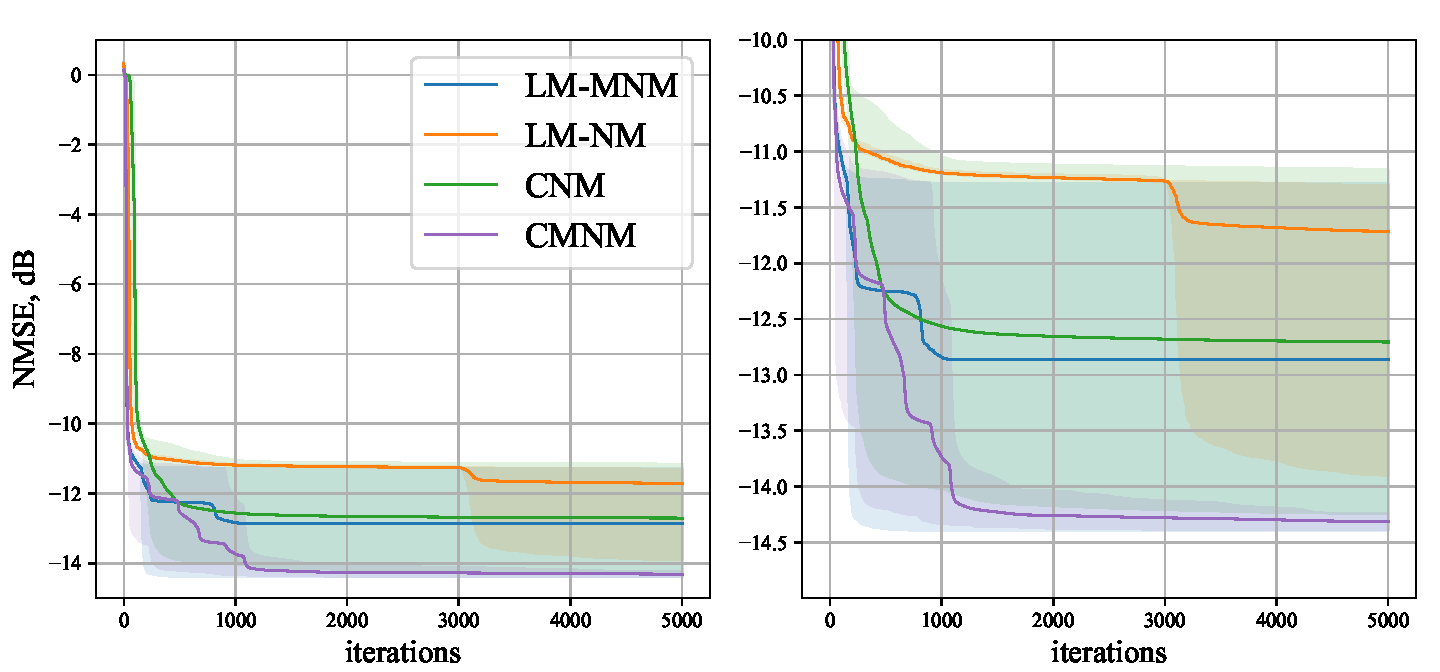
\includegraphics[scale=0.67]{figures/results/dpd_2ch_jota/learn_curves_cvcnn_all_algs.pdf}
%	\caption{Кривые сходимости методов второго порядка в задачу обучения комплекснозначной модели для компенсации нелинейных искажений в канале A двухканальной системы связи}
%	\label{fig:cv_cnn_learn_curves}
%\end{figure}
%\begin{figure}[h!]
%	\centering
%	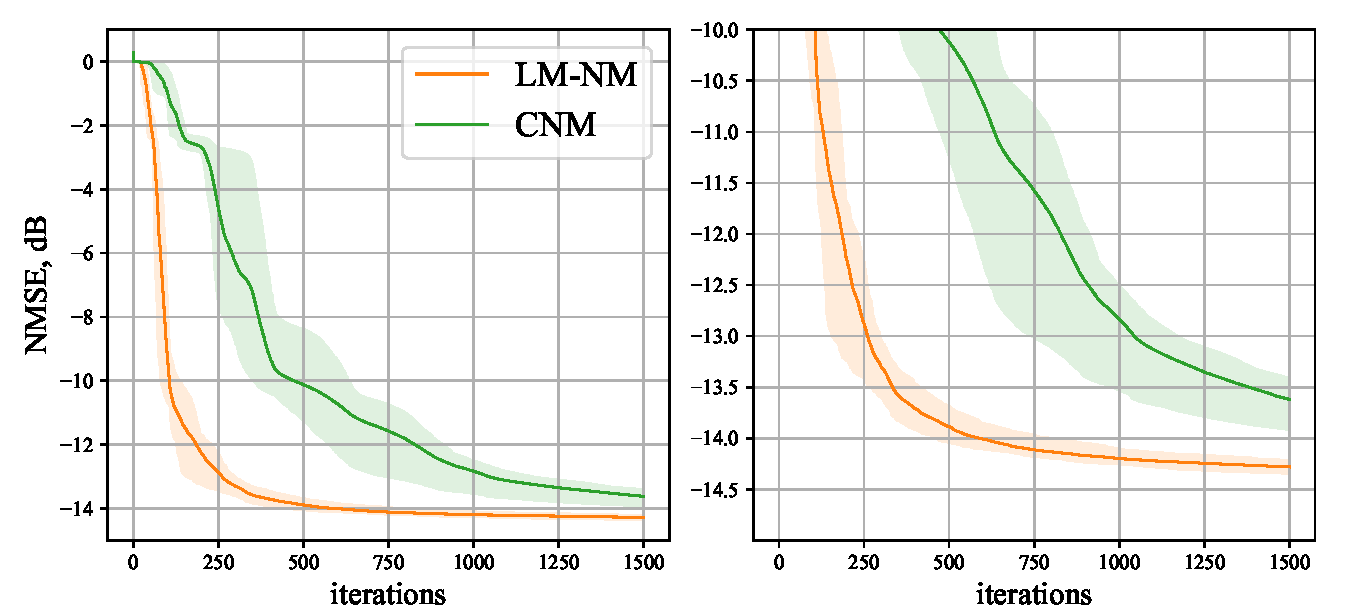
\includegraphics[scale=0.67]{figures/results/dpd_2ch_jota/learn_curves_rvcnn_all_algs.pdf}
%	\caption{Кривые сходимости методов второго порядка в задачу обучения вещественнозначной модели для компенсации нелинейных искажений в канале A двухканальной системы связи}
%	\label{fig:rv_cnn_learn_curves}
%\end{figure}
%\begin{figure}[h!]
%	\centering
%	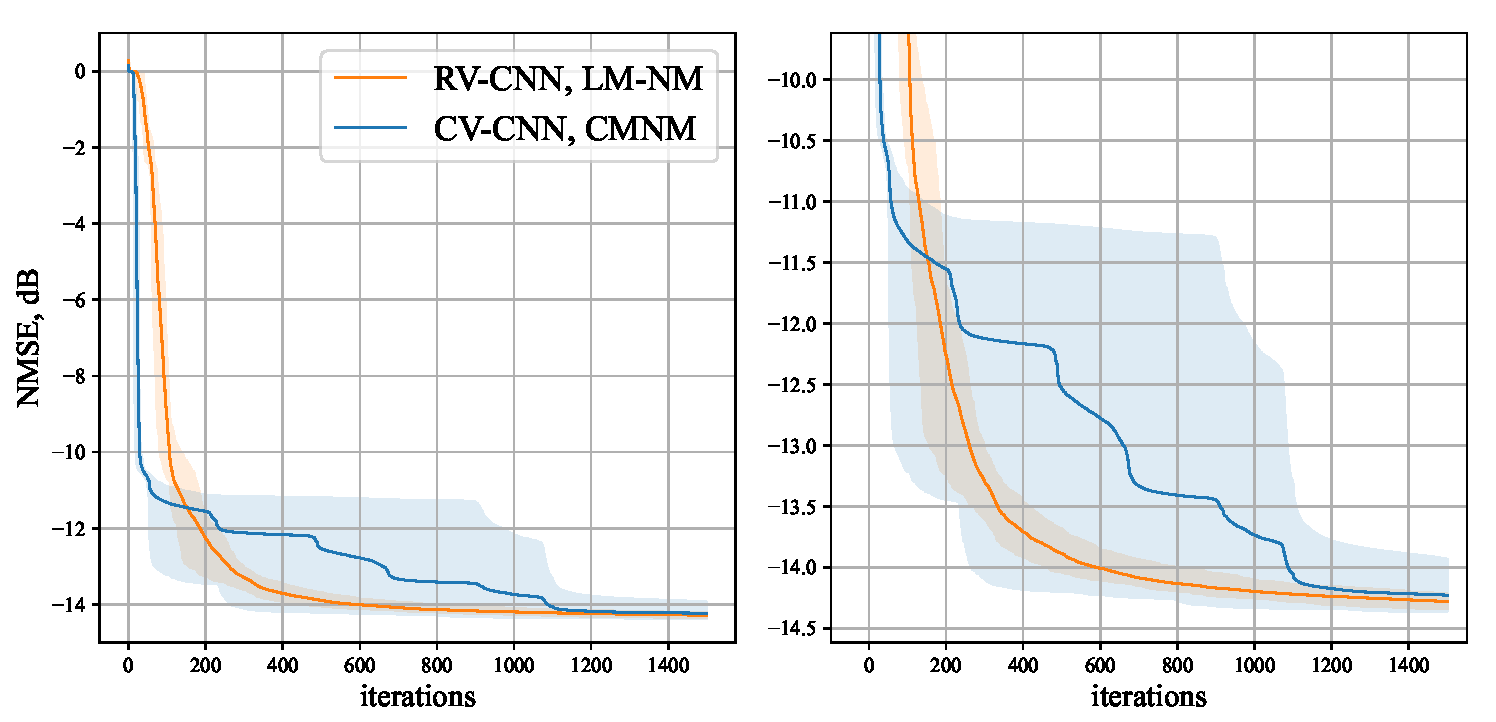
\includegraphics[scale=0.6]{figures/results/dpd_2ch_jota/learn_curves_both_models.pdf}
%	\caption{Сравнение кривых сходимости обучения моделей CV-CNN и RV-CNN}
%	\label{fig:cv_cnn_rv_cnn_learn_curves}
%\end{figure}
%
%Таблица~\ref{tab:dpd_2ch_converge_eval} отражает средние и минимальные значения критерия NMSE по всем начальным точкам для каждого алгоритма. Кроме того в таблице отражены относительные значения времени, затрачиваемого алгоритмами на один шаг адаптации.
%\begin{table}[ht]
%	\centering
%	\caption{Сравнение уровня компенсации и относительного времени сходимости рассмотренных методов}
%	\scalebox{0.95}{
%		\begin{tabular}{|c|c|c|c|c|c|c|}
%			\hline
%			& \begin{tabular}[c]{@{}c@{}}RV-CNN,\\ LM-NM\end{tabular} & \begin{tabular}[c]{@{}c@{}}RV-CNN,\\ CNM\end{tabular} & \begin{tabular}[c]{@{}c@{}}CV-CNN,\\ LM-NM\end{tabular} & \begin{tabular}[c]{@{}c@{}}CV-CNN,\\ CNM\end{tabular} & \begin{tabular}[c]{@{}c@{}}CV-CNN,\\ LM-MNM\end{tabular} & \begin{tabular}[c]{@{}c@{}}CV-CNN,\\ CMNM\end{tabular} \\ \hline
%			\begin{tabular}[c]{@{}c@{}}Относ. \\ усред. время  \\ на итер.\end{tabular} & 1 & 0.98 & 1.39 & 1.44 & \textbf{0.28} & 0.30 \\ \hline
%			\begin{tabular}[c]{@{}c@{}}Среднее\\ NMSE, \\ дБ\end{tabular} & \textbf{-14.28} & -13.62 & -11.71     & -12.71 & -12.87 & \textbf{-14.32} \\ \hline
%			\begin{tabular}[c]{@{}c@{}}Мин. \\ NMSE,\\  дБ\end{tabular} & \textbf{-14.34} & -13.91 & -13.91     & -14.25 & \textbf{-14.40} & \textbf{-14.39} \\ \hline
%	\end{tabular}}
%	\label{tab:dpd_2ch_converge_eval}
%\end{table}
%
%Кривые сходимости на рис.~\ref{fig:cv_cnn_learn_curves}, а также также результаты в таблице~\ref{tab:dpd_2ch_converge_eval} существенное преимущество смешанного метода Ньютона, построенного на кубической регуляризации. В среднем данный метод обеспечивает уровень компенсации лучше более чем на 2 дБ по сравнению с тремя другими рассмотренными методами. Кроме того, алгоритмы на основе смешанного метода Ньютона: LM-MNM, CMNM ускоряют скорость вычислений более, чем в 3 раза, что объясняется тем, что смешанный метод Ньютона не требует явного подсчета полной матрицы вторых производных (раздел~\ref{subsec:mnm} главы~\ref{chapter:intro}). Достаточно вычислить якобианы выходных векторов модели, а также их произведение.
%
%Кривые сходимости на рис.~\ref{fig:cv_cnn_rv_cnn_learn_curves} показывают, что в среднем скорость сходимости модели RV-CNN обучаемой методом Ньютона с регуляризацией на основе алгоритма Левенберга-Марквардта быстрее, чем скорость сходимости модели CV-CNN, обучаемой смешанным методом Ньютона с кубической регуляризацией. Тем не менее, обе модели в среднем сходятся к одному уровню компенсации (таблица~\ref{tab:dpd_2ch_converge_eval}) с разницей менее чем на 0.1 дБ. Кроме того, число вещественных параметров модели CV-CNN на основе комплексных параметров составляет $2\cdot109$ (таблица~\ref{tab:table_telecom_hyper}), что в 1.5 раза меньше числа обучаемых параметров вещественной модели при том же уровне компенсации.
%
%Спектральные плотности сигнала канала A на выходе услилителя мощности до включения нелинейного корректора и после изображены на рис.~\ref{fig:dpd_2ch_cnn_psd}.
%\begin{figure}[h!]
%	\centering
%	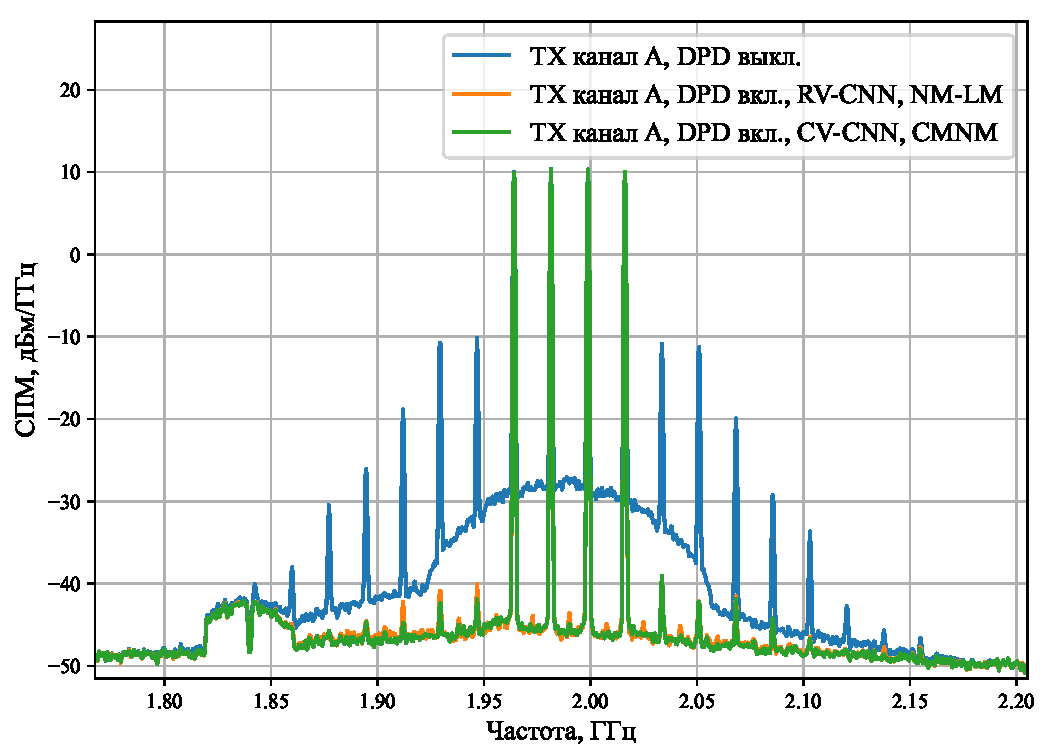
\includegraphics[scale=0.6]{figures/results/dpd_2ch_jota/psd.pdf}
%	\caption{Спектральные плотности мощности канала A на выходе УМ двухканальной системы до коррекции и после}
%	\label{fig:dpd_2ch_cnn_psd}
%\end{figure}
%Из рис.~\ref{fig:dpd_2ch_cnn_psd} видно, что уровни компенсации нелинейных искажений засчет адаптации обеих моделей RV-CNN, CV-CNN совпадает.
%
%Данный результат объясняется физической природой нелинейного преобразования. Поскольку нелинейные преобразования происходят над физическими электрическими сигналами, модель с кмоплексными параметрами является более физически-интерпретируемой. В связи с этим число параметров модели может быть выбрано меньше.
%
%Следует отметить, что вообще говоря смешанный метод Ньютона и его модификация с кубической регуляризацией не гарантирует глобальную сходимость. В сильно невыпуклых задачах, в особенности для случая многослойных нейронных сетей, данных метод может затревать в локальных оптимумах. 
%
%В связи с этим, требуется модификация смешанного метода Ньютона, которая позволит решить проблему локальных оптимумов. Прототипом для дальнейших исследований на эту тему может стать идея тяжелого шара "momentum", а также её модификация - алгоритм "Adam" (рассмотрены в разделе~\ref{subsec:grad_modified} главы~\ref{chapter:intro}). 
